\documentclass[a4paper,10pt]{article}
\usepackage{subfigure}
\usepackage{graphicx, epsfig}
\usepackage[numbers]{natbib}
\usepackage{german}
\usepackage[english]{mymacros_goerz}
\usepackage[
    pdftitle={Report on the Construction of the  PM2-Beamline at BESSY II},
    pdfauthor={Michael Goerz},
    pdfkeywords={BESSY II, Synchrotron, Beamline, X-Ray Source,
Insertion Devices, Undulators, Wigglers, Monochromator},
    colorlinks=true, 
    linkcolor=black, 
    urlcolor=black,
    citecolor=black,
    bookmarksopen=true,
    breaklinks=true
]{hyperref}


\begin{document}
\begin{titlepage}
    \centering
    \textsc{\LARGE Freie Universit"at Berlin \\[0.3cm]
Fortgeschrittenenpraktikum Physik}
    %   \vspace*{3.0cm}
    \rule{\linewidth}{0.5mm}\\[4.5cm]
    \textbf{\Large Report on the Construction of the  PM2-Beamline at BESSY II}
    \\[3.0cm]
    \begin{minipage}{0.4\textwidth}
        \begin{flushleft}
        {\Large \emph{Author:} \\[0.1cm] Michael Goerz}
        \end{flushleft}
    \end{minipage}
    \begin{minipage}{0.4\textwidth}
        \begin{flushright}
        {\Large \emph{Supervisor:} \\[0.1cm] Dr. Ralph P"uttner}
        \end{flushright}
    \end{minipage}
    \vfill
    \begin{minipage}{0.4\textwidth}
        \begin{flushleft}
        \centering
        \includegraphics[width=0.5\textwidth]{images/FUSiegel_sw_RGB.eps}
        \end{flushleft}
    \end{minipage}
    \begin{minipage}{0.4\textwidth}
        \begin{flushright}
        \centering
        \includegraphics[width=0.9\textwidth]{images/BESSYlogo.eps}
        \end{flushright}
    \end{minipage}
    \vfill
    \large{15. November 2007}
\end{titlepage}

\tableofcontents
\newpage


\def\abstractname{Summary}
\begin{abstract}
    This report describes the construction work that  Anton
Haase and I did on the PM2 beamline at BESSY II between April and July 2007. We
found the beamline in a semi-constructed condition and were able to bring it to
an almost operational status. The details of our work are described in Section
\ref{Description of the Construction Work}.

    Before that, I will give some background information on synchrotron
radiation and BESSY II in general in Sections \ref{Introduction}-
\ref{Operations at BESSY II}, followed by a review of the theoretical basics in
Section \ref{Theoretical Background}.
The report concludes with a documentation of the beamline's current status in
Section \ref{Layout of the PM2-Beamline}. There is an appendix describing the
control electronics for the monochromator.
\end{abstract}








\section{Introduction} \label{Introduction}

\begin{figure}[htbp]
    \centering
\includegraphics[width=0.9\textwidth]
{images/Schema_de_principe_du_synchrotron.eps}
    \caption{General Schematic of a Synchrotron}
  \label{image:Schema_de_principe_du_synchrotron}
\end{figure}

    In broad areas of physics and engineering, there is need for a source of
electromagnetic radiation, e.g. for  scattering experiments, excitation of
electronic states, microscopy, and a huge number of other applications.
Traditional light sources, such as X-ray tubes or simple discharge lamps, are
rather limited in their intensity, spectrum, continuity, and brilliance.
Additionally, researchers wish for a light source that can be used over a broad
spectrum instead of just specific wavelengths (e.g. lines of an X-ray tube). 

    These requirements can be fulfilled by synchrotron radiation. A synchrotron
is a specific type of particle accelerator, in which electrons are kept in
circulation at ultra-relativistic speeds -- i.e. effectively at the
speed of light -- by carefully placed strong magnets. Due to the well known
phenomenon of the emission of electromagnatic radiation
by charged particles undergoing acceleration, these accelerated electrons can
be used as a source for a wide variety of light from the visible part up to the
hard X-ray part of the spectrum: the necessary acceleration is produced by the
bending magnets keeping the electrons in their path. Additionally, there are
specialized \emph{insertion devices}, undulators and wigglers, which
produce alternative and variable radiation characteristics.

    \subsection{Historic Overview}

\begin{figure}[htbp]
    \centering
\includegraphics[width=0.7\textwidth]
{images/aerialview_1.eps}
    \caption{Aerial View of BESSY II}
  \label{image:aerialview_1}
\end{figure}

    BESSY II is a synchrotron of the third generation and has been in operation
since 1998. It replaced the second generation BESSY I (1982-1999), which had
been the first dedicated source of synchrotron radiation in Germany.

    Synchrotron radiation was first observed in 1947 by John Blewett at the
General Electrics Research Lab in Schenectady , New York\footnote{See
\citep{blewett1998} and \citep{robinson2000} for an introduction on the historic
origins.}, even though there had been theoretical work much earlier. Since the
observation was in a specific type of particle accelerator in which bunches of
electrons travel in a circle with a fixed radius -- a synchrotron, that
also became the name stuck to the radiation.

    Initially, synchrotron radiation was a major nuissance for the particle
accelerators, since it causes the particles to lose energy as they are forced
on their circular path. It took some years until the scientific potential of
the effect was recognized. The first experimental use of synchrotron
radiation for spectroscopy was not until about 10 years later (in 1956). First
research programs appeared in the 1960s.

    At first, researchers had to use the radiation that occurred as ``waste'' in
existing particle accelerators. These were the synchrotrons of the first
generation. With increased need, the first dedicated accelerators were built,
with the specific purpose of generating synchrotron radiation for experimental
needs. In these second generation facilities, the radiation produced at the
bending magnets was forwarded into beamlines. Finally, more specialized and
effective devices (undulators and wigglers) for the generation of synchrotron
radiation were developed. The modern third generation synchrotrons such as
BESSY II have long straight sections where these devices are put in place, in
addition to the traditional bending magnets. Recently, there is some development
towards forth generation devices, most notably the \emph{free electron laser},
which is also currently in planning at the BESSY II site.

    \subsection{Properties of Synchrotron Radiation}
    \label{Properties of Synchrotron Radiation}

    Synchrotron radiation has some properties that make it uniquely suitable
for scientific purposes:
\begin{itemize}
    \item broad spectrum
    \item high brilliance and great focusing conditions
    \item high intensity
    \item polarization
    \item pulsed
    \item highly predictable and controllable
    \item vacuum conditions
\end{itemize}

\begin{figure}[htbp]
    \centering
    \includegraphics[width=0.9\textwidth]{images/spektrum.eps}
    \caption{The Electro-Magnetic Spectrum, from
\citep{attwoodlecture}}
  \label{image:spektrum}
\end{figure}

    The first notable property is the wide spectrum that synchrotron radiation
encompasses. It includes the full range shown in Fig. \ref{image:spektrum}, from
the low infrared through visible light up to the hard X-rays, and may even
extend into somewhat lower and higher energies. It includes the primary
resonance energies of all elements.

\begin{figure}[htbp]
    \centering
\includegraphics[width=0.7\textwidth]{images/spectrum_characteristics.eps}
    \caption{Spectrum characteristics for Bending Magnets, Wigglers, and
Undulators}
  \label{image:spectrum_characteristics}
\end{figure}

    The specific spectrum characteristics depend on the insertion
device\footnote{I also count the bending magnets as insertion devices. Some
people differentiate between bending magnets and undulators/wigglers, referring
only to the latter two as insertion devices.}, as
shown in Fig.~\ref{image:spectrum_characteristics}. Bending magnets and wigglers
generate a broad frequency distribution, undulators have sharp peaks. The
insertion devices can be adapted for each beamline, and there will be
variable monochromators built in to achieve great flexibility.

    In all cases, the beam of synchrotron radiation is highly collimated, as is
often expressed by the \emph{brilliance}, one of the most characteristic
measures of quality:
\begin{eqnarray}
  B &=& \frac{N_f}{0.1\%, \milli\meter^2 \milli\radian^2}
\end{eqnarray}
The brilliance is defined as the number of photons per second ($N_f$) per 0.1\%
bandwidth per area per solid angle.\footnote{
See \citep{eriksson1997}. This
quantity is sometimes also called \emph{spectral brightness}. It is also
sometimes expressed at power per bandwith, area, and solid angle (See
\citep{attwood2000}). For a comment on the ambiguity of nomenclature, see
\citep{mills2005}.
} For experimental purposes, the high brilliance translates
into a high intensity of the synchrotron light.

    Due to the design of the insertion devices, the synchrotron radiation has
linear or elliptical polarization. Also, since the electrons travel in very
localized bunches\footnote{This is due to the workings of the accelerator, which
will be explained in Section \ref{Operations at BESSY II}.}, the radiation that
the experimentalist sees is pulsed. At BESSY II, the frequency is 500
$\mega\hertz$, with each pulse lasting 0.02 $\nano\second$.

    The theory of synchrotron radiation (see Section 
\ref{Theoretical Background}) is very well understood and allows very precise
calculation of the radiation characteristics. The insertion devices can be
manufactured and adapted with equal precision, so that for each experiment, the
conditions are highly controllable. It is this precision and flexibility -- each
beamline can receive the exact desired radiation due to the use of insertion
devices -- that separates third generation synchrotrons from earlier setups.

    Lastly, the entire synchrotron operation including the beamlines has to
take place in an ultra-high-vacuum environment; maintaining an electron beam
would be impossible otherwise. This has the added benefit that researchers do
not have to worry about their samples becoming contaminated in an atmosphere.

    \subsection{Applications}

    There is a wide variety of research from different fields of science and
engineering taking place at BESSY II, which illustrates the importance of
synchrotron light sources.

    The original report proposing the construction of BESSY II \citep{bessy}
already takes 50 pages to explicate the intended uses in eight different
categories. 

    In atomic and molecular physics, the broad spectrum is suitable for a
detailed spectroscopy of energy levels, among many other things. The high
intensity is needed to work with low-density (non-solid-state) samples. 

    In chemistry, a number of processes can be examined, such as photochemical
processes, in which the light is used to manipulate chemical bondings, dynamic
processes that need rapid pulse and highly intense radiation, and spectroscopy
of clusters (systems of few atoms). 

    Listed next is matrix isolation spectroscopy, in which atomic structures
(atoms, molecules, clusters) are insterted at low temperatures into a host
grid, which isolates and stabilizes them, allowing detailed chemical analysis.

    In solid state physics, the spectroscopy with photo-absorption and
-emission requires a tunable light source. There is a research group at BESSY II
working within the solid state field on magnetic nano-structures.

    For the physics of surfaces and interfaces, most of the spectroscopic
methods used in solid state physics can also be used in a surface sensitive
mode. However, a high intensity of radiation is needed, as well as the spacial
and spectral resolution that the synchrotron can provide.

    Another important field is X-ray microscopy. The resolution of optical
microscopes is limited by the wavelength of the used light, so that short
wavelength X-rays can provide a major improvement. This method has some
benefits to alternatives such as electron microscopy, which places severe
restrictions on the samples.

    The Physikalisch-Technische-Bundesanstalt (PTB) uses BESSY II for various
tasks of radiometry. They define standards of measurement, as well as test and
calibrate industrial products. Because the synchrotron light source is so
controllable, it can serve as a standard.

    Lastly, there are several other industrial applications, most notably in
the microengineering field. The Anwenderzentrum f"ur Mikrotechnik (AZM) uses
the excellent light characteristics for X-ray lithography for the engineering
of nano-structures.

    All of these tasks, among some others, are currentely being worked on at
BESSY II. The BESSY website\footnote{\url{http://www.bessy.de}} and
the ``Highlights'' brochure \citep{bessy_highlights2006} inform about current
research activities. Most notable beyond the ones mentioned above are the
installation of an infra-red beamline, which is used for the spectroscopy of
biological samples as well as some other purposes. There is also a lot of
activity at the development of new generation synchrotrons. The insertion
devices are in constant development, and as a long term project, the free
electron laser \citep{bessyfel} is planned as an addition to the
facility.

    The breathtaking multitude of all the projects, which I can only list here
without much explanation, shows how important synchrotron radiation is as a
tool of scientific research.








\section{Operations at BESSY II} \label{Operations at BESSY II}

    We can now look in some detail at how synchrotron radiation is produced and
delivered at the beamlines. Fig.~\ref{image:beamlines_map_annotated} shows a
detailed map of the facility, including all beamlines\footnote{You may also go
back to Fig.~\ref{image:Schema_de_principe_du_synchrotron} for comparison, it
depicts the same basic synchrotron structure, leaving out wigglers and
undulators}. We will follow the steps 1-8 as they are labeled in the figure.
A brief outline of the electron beam generation and acceleration
appears in \citep{kramer1993}.

\begin{figure}[htbp]
    \centering
    \includegraphics[width=\textwidth]{images/beamlines_map_annotated.eps}
    \caption{Detailed Map of Ring Structure and Beamlines at BESSY II}
  \label{image:beamlines_map_annotated}
\end{figure}

    \subsection{Electron Generation}

    At step (1), electrons are generated from a simple filament in a vacuum
tube, and are first accelerated by the anode voltage in the tube. They then
enter a \emph{racetrack microtron}, which works as shown in
Fig.~\ref{image:racetrack_microtron}. The microtron is a simple but effective
device, in which the electron beam is passed through a linear accelerator (red
tube) repeatedly. After each pass, the beam is turned {180\degree} by a
magnetic field (green). As the electrons' kinetic energy increases, they spiral
outwards, but still go through the accelerator each cycle. Finally, when they
have reached their maximum energy, {50 \mega\electronvolt}, they leave the
microtron.

\begin{figure}[htbp]
    \centering
\includegraphics[width=0.7\textwidth]{images/racetrack_microtron.eps}
    \caption{Racetrack Microtron, from \citep{mainz_prospekt}}
  \label{image:racetrack_microtron}
\end{figure}



    \subsection{The Synchrotron Ring}
    So far, we have referred to the entire BESSY II or similar facilities as
``synchrotron''. This is common usage, but not entirely correct. The term
synchrotron does in fact refer to a specific circular type of
\emph{accelerator}, which is the next step (2) in the processing of the
electron beam. The synchrotron is only the smaller inner circle of {96
\meter} circumference, whereas the large outer circle with {240 \meter}
circumference to which the beamlines are connected is properly called
the \emph{storage ring}.

    In the synchrotron ring, the electrons are accelerated to their final
energy of {1.7 \giga\electronvolt} (max. {1.9 \giga\electronvolt}). The
acceleration happens through cavity resonators (see Section 
\ref{Microwave Cavity Accelerators}), and the electrons are kept in their
circular paths by regular bending magnets. 

    The bending magnets are simple dipole magnets, similar to the storage ring
dipole magnets shown in Fig.~\ref{image:dipoles_combined}. They have a
homogeneous magnetic field, so that the electron is forced on a circular path
with radius
\begin{eqnarray}
  r &=& \frac{v \cdot \gamma \cdot  m_e}{e \cdot B}. \label{eq:bend_mag_radius}
\end{eqnarray}



\begin{figure}[htbp]
    \centering
\includegraphics[width=0.9\textwidth]{images/dipoles_combined.eps}
    \caption{Storage Ring Dipole Magnets, from \citep{becker1995}}
  \label{image:dipoles_combined}
\end{figure}

    As the speed of the electrons increases and approaches the speed of light,
the magnets have to adapt with an increased magnetic field. This is what
separates the synchrotron ring from the storage ring. The synchrotron ring is
purely an accelerator, which is used only for brief periods, whereas in the
storage ring, the electrons are kept at a constant speed for an extended period
of time (several hours). The beamlines rely on the constant energy of the
electron beam in the storage ring.

    \subsection{Injection}
    When the electron beam has reached its final velocity, it is injected
into the storage ring at step (3). For this purpose, a carefully timed
\emph{kicker} magnet deflects the electron beam out of the synchrotron ring into
the injection line, with another kicker pushing it into the storage ring.

    \subsection{Focusing}

\begin{figure}[htbp]
    \centering
    \includegraphics[width=0.7\textwidth]{images/quadrupol.eps}
    \caption{Sketch of a Quadrupole Bending Magnet, from \citep{wille1991}}
  \label{image:quadrupol}
\end{figure}

    Once in the storage ring, the electron beam is kept in circulation for
up to ten hours. To keep the beam stable during this time, and to compensate for
aberrations caused by the dipole magnets and other insertion devices, it is
important to keep the electron beam focused. This is done with multipole
magnets. The different magnetic devices and their parameters are available in
\citep{becker1995, budz2006}.

    The simplest layout, a quadrupole magnet, is shown in
Fig.~\ref{image:quadrupol}. It is easy to see that the electron beam is pushed
back to the center (perpendicular to the magnetic field lines) if it deviates
from the center.

    Other multipole magnets are used in a similar vein; they can have more
specialized properties such as the compensation of chromatic errors. 

    A magnetic focusing element is labeled as step (4) in
Fig.~\ref{image:beamlines_map_annotated}

    \subsection{Insertion Devices} \label{Insertion Devices}


\begin{figure}[htbp]
    \centering
    \includegraphics[width=0.7\textwidth]{images/undulator_detailed.eps}
    \caption{Schematic of and Undulator/Wiggler, from \citep{attwoodlecture}}
  \label{image:undulator_detailed}
\end{figure}

% \begin{figure}[htbp]
%     \centering
%     \includegraphics[width=0.8\textwidth]{images/undulator_wiggler.eps}
%     \caption{Undulators vs. Wigglers}
%   \label{image:undulator_wiggler}
% \end{figure}

    In order to extract the synchrotron radiation from the storage ring,
insertion devices (IDs) are used. This can be bending magnets (5), undulators
(6), or wigglers (7). Additionally, there are some wavelength shifters in use at
BESSY II. Each ID has different radiation characteristics, as discussed in
Section \ref{Properties of Synchrotron Radiation}.

    Undulators and wigglers are very similar in their setup. They both use an
array of magnets to oscillate the electron beam in a sine-wave (or on an
elliptical path for a more complicated variation). As the electrons are
accelerated during this process, they emit synchrotron radiation. The principal
difference between wigglers and undulators is the strength of the magnets, which
corresponds to the amplitude of the oscillations. Undulators use magnets that
are approximately as strong as the bending magnets in the storage ring, and
therefore only produce smaller oscillations. Wigglers use much stronger fields,
generated with superconducting coils. Specifically, the distinction is made
according to the \emph{wiggler strength}
\begin{eqnarray}
  K &=& \frac{e \lambda_u B_0}{2 \pi m c^2}.\label{eq:undulator_wiggler_k}
\end{eqnarray}
$B_0$ represents the maximum magnetic field, $\lambda_u$ the wavelength of the
sine path, as shown in Fig.\ref{image:undulator_detailed}. Large
values of $K$ describe wigglers, small numbers ($K=1.5$)
describe undulators.

    The difference in terms of the radiation characteristics can be seen in
Fig.~\ref{image:undulator_wiggler_overlap}. Due to the extreme deflection of
the beam in the wiggler case, the synchrotron radiation cones are spread over a
larger space and do not overlap significantly. This leads to a broad spectrum,
similar to bending magnets. However, the intensity is much higher, with the
electron beam being wiggled over multiple (sine) cycles. A bending magnet in
comparison only emits radiation from the fraction of a cycle (the fraction of
the bending magnet length to the full storage ring circumference) 

    In the undulator case, the deflection is much smaller, and the radiation
cones overlap, causing them to interfere. This leads to a peak in the spectrum
(the maximum of constructive interference) in addition to a high intensity.

    An additional aspect is polarization. In the simplest case, which we
discussed, the polarization of the synchrotron radiation is linear. With more
complicated undulator and wiggler setups, where the electrons are forced on a
spiral, elliptical polarization can also be obtained.


\begin{figure}[htbp]
    \centering
    \includegraphics[width=0.8\textwidth]{images/undulator_wiggler_overlap.eps}
    \caption{Undulator and Wiggler Radiation, from \citep{bessy}}
  \label{image:undulator_wiggler_overlap}
\end{figure}

    The ID in use for the PM2 beamline is a simple dipole bending magnet.


    \subsection{Microwave Cavity Accelerators}
    \label{Microwave Cavity Accelerators}

\begin{figure}[htbp]
    \centering
    \includegraphics[width=0.6\textwidth]{images/microwave_accel.eps}
    \caption{Principle of Microwave Cavity Accelerator, from \citep{wille1991}}
  \label{image:microwave_accel}
\end{figure}

    Each insertion device extracts energy from the storage ring (the energy of
the synchrotron radiation). To compensate for this, the beam has to be
accelerated slightly at each cycle to maintain its speed. Additionally, the
electrons traveling in a bunch smear out over time and have to be recompressed.
Both tasks are fulfilled with a microwave cavity resonator at step (8).

    Inside the resonator, there is a standing microwave with a frequency of 500
\mega\hertz. As depicted in Fig.~\ref{image:microwave_accel}, the electron beam
enters the resonator at a nominal phase $\Psi_0$ of the oscillation, and is
accelerated by the energy $e \cdot U_0$. Electrons arriving too late
($\frac{\Delta P}{P} < 0 $) see a higher voltage ($ U = U(\Psi - \Delta \Psi)$),
those arriving too early ($\frac{\Delta P}{P} > 0 $) a higher one. In this way,
the nominal energy of the electron beam is enforced, and the loss due to
synchrotron radiation is replenished.

    Nonetheless, the time the electron beam can be kept stable in the storage
ring is limited, at some point the electrons will collide with each other
or scatter on the few remaining molecules left in the pipe (imperfections of
the vacuum conditions).

    \subsection{Beamlines}
    \label{Beamlines}

\begin{figure}[htbp]
    \centering
    \includegraphics[width=0.8\textwidth]{images/typical_beamline.eps}
    \caption{A Typical Beamline, from
\citep{attwoodlecture}}
  \label{image:typical_beamline}
\end{figure}

    Once the synchrotron radiation is generated at the insertion device, the
beamline takes the task of adapting the radiation to the experimental needs.
This especially means monochromatization and focusing. A typical beamline is
shown in Fig. \ref{image:typical_beamline}.

    For bending magnet radiation, all adaptions have to be made within the
beamline, while for wigglers and especially for undulators, the parameters
(magnetic field, distance between magnetic poles) can be tweaked to produce
radiation with the desired characteristics.

    Note that for the wavelengths that are typically used, transmission optics
such as lenses are no longer feasible. Instead, long curved grazing mirrors are
use to focus the beam (M1, M2 in Fig. \ref{image:typical_beamline}), and
adjustable gratings provide the monochromatization. 

    One of the problems that has to be dealt with for the optics is the heat
that is due to the high intensity of the synchrotron radiation. For some
beamlines, the optical parts have to be water-cooled.

    The workings of the PM2 beamline will be described in more detail in Section
\ref{Layout of the PM2-Beamline}.


\section{Theoretical Background} \label{Theoretical Background}

    \subsection{Radiation of Charges in Circular Motion}
    The theory behind synchrotron radiation is that of a charge moving at
relativistic speed. A thorough theoretic discussion of this can be found in
\citep[Chapter 14]{jackson1999}. A comprehensive theoretical overview
of all the aspects of the synchrotron operation appears in \citep{wille1991}.

    The starting point is the radiation of a non-relativistic accelerated
charge with its wellknown $\sin^2\theta$-dependancy. This is the case that is often
used to describe antennas, for example. With $\vec{\beta} = \frac{\vec{v}}{c}$
and $\vec{n}$ being the radial unit vector (pointing in direction of the observer), the power per solid angle
is: \footnote{cf. \citep[p. 665]{jackson1999}}
\begin{eqnarray}
  \difquo[P]{\Omega} 
  &=& \frac{e^2}{4 \pi c} 
     \left|\vec{n} \times (\vec{n} \times \dot{\vec{\beta}}) \right|^2 
     \label{eq:angular_power_nonrelativistic}\\
  &=& \frac{e^2 }{4 \pi c^3}|\dot{\vec{v}}|^2 \sin^2 \theta 
\end{eqnarray}

    In the case of relativistic speed, this formula needs to be adapted. To
find the formula describing our case, one has to go back to the Lienard-Wiechert
theory of retarded potentials, and look at the radial component of the Poynting
vector that comes forth from this analysis:
\begin{eqnarray}
  [\vec{S} \cdot \vec{n}]_{\text{ret}}
  &=& 
  \frac{e^2}{4 \pi c}
    \left\{
       \frac{1}{R^2} \left|
         \frac{
             \vec{n} \times [  (\vec{n} - \vec{\beta}) \times
             \dot{\vec{\beta}}  ]
            }
            {
             (1-\vec{\beta}\cdot \vec{n})^3 
            }
       \right|^2
   \right\}_{\text{ret}}\label{eq:poynting_nonrelativistic}
\end{eqnarray}
$R$ is the distance between the reference point and the position the charge had
when it first emitted the radiation that is now visible at the reference
point (in the picture of the relativistic light-cone).

    From this we get to the power per unit solid angle in the time-frame $t'$ of
the electron ($t' = t - R(t')/c$):
\begin{eqnarray}
  \difquo[P(t')]{\Omega}  
    &=& R^2 \vec{S} \cdot \vec{n} \;  (1-\vec{\beta}\cdot\vec{n}) \\
    &=& \frac{e^2}{4 \pi c}
        \frac
           {\left| \vec{n} \times 
            \{ 
              (\vec{n} - \vec{\beta}) \times \dot{\vec{\beta}} 
            \} \right|^2
           }
           {
             (1- \vec{n} \cdot \vec{\beta})^5
           } \label{eq:angular_power_relativistic}
\end{eqnarray}
Note how Eq. (\ref{eq:angular_power_relativistic}) turns into Eq.
(\ref{eq:angular_power_nonrelativistic}) for $\beta \ll 1$

\begin{figure}[p]
    \centering
    \includegraphics[width=0.9\textwidth]{images/searchlights.eps}
    \caption{Radiation Cones for Increasing Speeds (arbitrary units)}
  \label{image:searchlight}
\end{figure}

\begin{figure}[p]
    \centering
    \includegraphics[width=\textwidth]{images/fullpolar.eps}
    \caption{Radiation Cone for $v=0.98c$}
  \label{image:fullpolar}
\end{figure}

    We can now look at a circular relativistic motion, i.e. $\vec{\beta} \perp
\dot{\vec{\beta}}$ and get (with $\Theta$ measured from the direction of
$\vec{v}$):
\begin{eqnarray}
  \difquo[P(t')]{\Omega}
  &=& \frac{e^2}{4 \pi c^3}
      \frac{|\dot{\vec{v}}|^2}{(1-\beta \cos \Theta)^3}
      \left[
        1 - \frac{
          \sin^2 \Theta \cos^2 \Phi
        }{
          \gamma^2 (1-\beta \cos \Theta)^2
        }
      \right] \label{eq:angular_power_relativistic_circular}
\end{eqnarray}
Fig. \ref{image:searchlight} shows how $\difquo[P]{\Omega}$ develops for
increasing relativistic speed. At rest, there is again the classic $\sin^2 \theta$
picture. With $\beta = v/c$ going from 0 to 1, the forward pointing lobe
inflates massively. The cone pointing backwards at $\beta = 0$ is also pulled
in the forward direction (the points of zero emission move from $\pi/2$ to a
lower angle). Fig. \ref{image:fullpolar} shows the full radiation cone at a
speed of 98\% the speed of light, which is not nearly the speed the electrons
have in the storage ring. Obviously, the radiation peaks very sharply in the
direction of the movement, i.e. in radial direction from the storage ring. It
will appear as a ``searchlight'' whenever the electron beam passes the bending
magnet.

    There is also a more intuitive explanation to the searchlight property than
derivating Eq. (\ref{eq:angular_power_relativistic}). The change from a $v=0$ to
$v=c$ can also be understood in terms of the relativistic Doppler effect. For
an observer looking at the incoming electron beam, the wavelength is
massively shortened. i.e. the energy is massively enlarged.  Using the
relativistic Doppler effect, it is possible to quantify the narrowness of the
cone (i.e. the directedness of the radiation): With the z-Axis pointing in the
direction of the movement, and $\vec{k}'$  being the wave vector in the
electron's frame of reference and $\vec{k}$ being the wavefactor in the
laboratory frame of reference, we can look at $\Theta \approx \frac{k_x}{k_z}$.
The Doppler stretching of the wave vector only occurs in z-direction, so $k_x =
k_x'$. For $k_z$ we have
\begin{eqnarray}
  k_z &=& \frac{2 \pi}{\lambda} \\
  \lambda &=& \lambda' \sqrt{\frac{1-\beta}{1+\beta}} \qquad
     \text{cf. \citep{weisstein_doppler}} \nonumber \\
          &=& \lambda' \frac{\sqrt{1-\beta^2}}{1+\beta} \nonumber \\
          &=& \lambda' \frac{1/\gamma}{1+\beta} \nonumber \\
          &\approx& \lambda' \frac{1}{2 \gamma} \qquad 
             \text{for $\beta\rightarrow 1$} \\
  k_z &\approx& 2 \gamma k_z'
\end{eqnarray}
This gives us the stretching of a reference angle $\Theta' =
\frac{k_x'}{k_z'} = 1$, i.e. the width of the synchrotron radiation:
\begin{equation}
  \Theta \approx \frac{k_x}{k_z} 
         \approx \frac{k_x'}{2 \gamma k_z'} 
            =     \frac{1}{2 \gamma} \label{eq:theta_width}
\end{equation}

    \subsection{Bending Magnet Radiation}
    The formulas presented so far describe the general case of accelerated
electrons moving in a circle. As such, they directly describe the radiation of
bending magnets, but are equally the foundation of the other IDs in which the
acceleration is a sine wave. The radiation of charges that are not moving in a
circle can be described by applying the above formulas to the (circular)
curvature at each point and looking at the superposition of the radiation from
all the individual points.

    In addition to the directedness and high intensity that Eq.
(\ref{eq:angular_power_relativistic_circular}) proves for high speeds,
Section \ref{Properties of Synchrotron Radiation} also mentioned the broad
spectrum of synchrotron radiation (for bending magnets and wigglers). A good
theoretical explanation\footnote{following \citep{attwood2000}}, albeit
somewhat handwaving, comes from the use of the Heisenberg uncertainty
principle.

    \begin{eqnarray}
      \Delta E \cdot \Delta \tau &\geq& \hbar / 2
    \end{eqnarray}

\begin{figure}[htbp]
    \centering
    \includegraphics[width=0.6\textwidth]{images/pulseduration.eps}
    \caption{Pulse Duration for Bending Magnet Radiation, from
\citep{attwood2000}}
  \label{image:pulseduration}
\end{figure}

    In  order to calculate $\Delta E$, we first have to find an expression for
$\Delta \tau$, which we can get from looking at
Fig.~\ref{image:pulseduration}. Following the convention usually followed by
synchrotron physicists, the half-width of the radiation pulse is $2 \Delta
\tau$ (Fig.~\ref{image:pulseduration}(b)). The geometry is presented in
Fig.~\ref{image:pulseduration}(a); with the width of $\theta$ as in
Eq. (\ref{eq:theta_width}), an observer will see radiation while the electrons are
between point A and point B, i.e. for the time that the electrons need to
travel that distance minus the time the radiation itself needs to travel from A
to B. We therefore get
\begin{eqnarray}
  2 \Delta \tau 
    &\approx& \frac{R \cdot 2 \Theta}{v} - \frac{2R \sin \Theta}{c} \nonumber \\
    &\approx& \frac{R}{\gamma}{\frac{1}{v} = \frac{1}{c}}
\end{eqnarray}
With Eq. (\ref{eq:bend_mag_radius}) and 
\begin{eqnarray}
  (1-\beta) &\approx& \frac{1}{2\gamma^2}
\end{eqnarray}
we get
\begin{eqnarray}
  2 \Delta \tau 
    &\approx& \frac{m}{2eB\gamma^2}
\end{eqnarray}
and therefore
\begin{eqnarray}
  \Delta E &\geq& \frac{2 e \hbar B \gamma^2}{m}.
\end{eqnarray}

    A rather complicated theoretical analysis\footnote{cf. \citep{hofmann2004}}
can provide a formula for the flux of photons of energy $E$ in a given solid
angle and bandwidth:

\begin{eqnarray}
  \left.\frac{\dd^3 F_B}{\dd \Omega \dd \phi \dd \omega/\omega}\right|_{\phi=0}
  &=& 1.33 \cdot 10^{13}\cdot  E_e^2 \cdot I 
      \cdot (\frac{E}{E_c})^2 \cdot  K^2_{2/3}\left(\frac{E}{2E_{c}}\right)
\end{eqnarray}
where $E_e$ is the energy of the electron beam in {\giga\electronvolt}
({1.7 \giga\electronvolt} for BESSY II), $I$ is the current in the ring in
{\milli\ampere} ({100 \milli\ampere}), $E_c$ is the critical photon energy -- the
energy at which half the power is emitted at lower energy and half at higher
energy:
\begin{eqnarray}
  E_c &=& \frac{3 e \hbar B \gamma^2}{2m}
\end{eqnarray}
The $K_{2/3}$ are modified Bessel-functions.

    By integrating over the azimuthal angle $\phi$ on gets a more commonly used
expression for the flux that is plotted in Fig. \ref{image:flux}
for the parameters of the BESSY ring:\footnote{Compare this with
\url{http://www.bessy.de/upload/insertion_devices/files/flux.pdf}}

\begin{eqnarray}
  \frac{\dd^2 F_B}{\dd \Omega \dd \omega/\omega}
  &=& 2.46 \cdot 10^{13}\cdot  E_e^2 \cdot I 
      \cdot (\frac{E}{E_c})^2 \cdot G\left(\frac{E}{2E_{c}}\right)
\end{eqnarray}
with
\begin{eqnarray}
  G(x) &:=& x \cdot \int_{x}^{\infty} K_{5/3}(x') \dd x'.
\end{eqnarray}

\begin{figure}[htbp]
    \centering
    \includegraphics[width=0.6\textwidth]{images/flux.eps}
    \caption{Flux in photons per second and 0.1\% bandwidth for $E_e = 1.7 \,
\giga\electronvolt$ and I = 100 \,
\milli\ampere}
  \label{image:flux}
\end{figure}

    \subsection{Undulators and Wigglers}
    The concept of undulators and wiggles was already explained in Section
\ref{Insertion Devices}. The undulator achieves its characteristic peak in the
spectrum due to the constructive interference of the coherent radiation that is
thrown off at each oscillation. There are higher modes of that peak, but in
almost all cases only the \emph{central cone} is used.

    While the formulas for the undulators are important for synchrotrons in
general, since the PM2 beamline has a bending magnet as an insertion device, I
will not go into as much detail with their derivation.

    Most important is the \emph{undulator equation} that calculates the peak
wavelength:
    \begin{eqnarray}
      \lambda &=&\frac{\lambda_u}{2 \gamma^2} 
                 \left(
                   1 + \frac{K^2}{2} + \gamma^2 \Theta^2
                 \right) \label{eq:undulator_equation}
    \end{eqnarray}
with $K$ as defined in Eq. (\ref{eq:undulator_wiggler_k}) and $\lambda_u$ being
the undulator period. The term $\frac{\lambda_u}{2 \gamma^2}$ comes out of the
relativistic Doppler effect, $\frac{K^2}{2}$ accounts for the transverse
motion in the undulator, and $\gamma^2 \Theta^2$ is a correction for the
radiation off axis.

    The peak width is described as:
\begin{eqnarray}
  \frac{\Delta \lambda}{\lambda} &=& \frac{1}{N} \label{eq:undulator_bandwidth}
\end{eqnarray}
This can be seen when looking at the situation as a Fourier transform: $1/N$ is
generally the width of the Fourier transform of $N$ harmonic cycles. In
retrospect, the Fourier transform picture also gives an explanation of why the
bending magnet spectrum is so broad: the electron in this case only makes a
fraction of a cycle (one full cycle is the entire storage ring). In wigglers,
contrary to the undulator case, the radiation does not overlap coherently, so
there is no peak, but a broad spectrum like for the bending magnets.

    We can now look at the opening angle of the cone that would include the
bandwidth of Eq. (\ref{eq:undulator_bandwidth}). By taking Eq.
(\ref{eq:undulator_equation}) once off axis ($\Theta \neq 0$)  and once on
axis ($\Theta = 0$) and dividing the two expressions, one can see that
\begin{eqnarray}
  \frac{\Delta \lambda}{\lambda} &\approx& \gamma^2 \Theta^2
\end{eqnarray}
By demanding that for $\Theta = \Theta_{\text{cent}}$ Eq.
(\ref{eq:undulator_bandwidth}) holds, we get
\begin{eqnarray}
    \Theta_\text{cen} &\approx& \frac{1}{\gamma\sqrt{N}}
\end{eqnarray}
This is the undulator equivalent to Eq. (\ref{eq:theta_width}).

    Finally, the power radiated in the central cone can be calculated as:
\begin{eqnarray}
  \bar{P}_{\text{cent}} &\approx& \frac{\pi e \gamma^2 I}{\epsilon_0 \lambda_u}
                                  \frac{K^2}{(1 + \frac{K^2}{2})^2}
\end{eqnarray}

    For wigglers, there are no new fundamental new formulas as compared to
the bending magnets. The main difference is the higher intensity, and some
adjustability of the parameters.


\section{Description of the Construction Work} 
\label{Description of the Construction Work}

The beamline as we found it was complete in its major parts, but was still
missing some larger pieces in its second half. The full beamline is shown in
Fig. \ref{image:beamline}, with the parts that we had to add or modify
significantly highlighted in red.

\begin{figure}[htp]
  \begin{center}
    \subfigure[Ground Attachment]{
      \label{image:constr01a}
      \includegraphics[width=0.5\textwidth]{images/constr01a.eps}}
    \subfigure[Mounting Structure]{
      \label{image:constr01b}
      \includegraphics[width=0.4\textwidth]{images/constr01b.eps}}
  \end{center}
  \caption{The Supporting Pillars}
  \label{image:constr01}
\end{figure}

    The first task was to put in the supporting pillars (Fig.
\ref{image:constr01}). The exact track of the beamline was measured out and
marked on the ground by the BESSY staff. Since the beamline has to follow the
radiation beam exactly, it is important to have a very precise layout and
measurement of the beamline construction. To facilitate this precision, there is
a special coordinate system for the entire experimentation hall.

    The pillars are screwed to the floor. For this, three holes we drilled
for each pillar and filled with a special glue to hold the screw anchor (Fig.
\ref{image:constr01a}). This provided an extremely stable and permanent basis
for the pillars. The hollow steal pillars were filled with sand for added
weight, and then the mounting structure (Fig. \ref{image:constr01b})  had to be
assembled on top. The structure is adjustable in height and can rotate
horizontally.

\begin{figure}[htp]
  \begin{center}
    \subfigure[Mounted Pipes]{
      \label{image:constr02a}
      \includegraphics[width=0.48\textwidth]{images/constr02a.eps}}
    \subfigure[Pipe Connection]{
      \label{image:constr02b}
      \includegraphics[width=0.48\textwidth]{images/constr02b.eps}}
  \end{center}
  \caption{Assembly of the Pipes}
  \label{image:constr02}
\end{figure}

    Next, we put in the two-meter connecting pipes, as shown on Fig.
\ref{image:constr02}. One has to take care to keep the inside of the pipes and
all other parts clean, as they will have to provide an ultra-high-vacuum that
would be difficult to achieve with significant amounts of dust inside the
beamline. Hence all open connectors were covered with plastic (or aluminum
foil) caps.

    The junction between two pipes, or any two parts in general was done with
an abundant number of screws. A copper gasket ring was placed between the two
connectors. Copper, as a soft metal, dents under the pressure of the junction
and ensures that the construction can hold a vacuum. It takes some practice to
make a junction, since the copper rings will not always stay in place easily.
Also, special care has to be taken to close all the screws firmly but evenly.
Otherwise, leaks may occur.

\begin{figure}[htbp]
  \begin{center}
    \subfigure[Assembly of a Pump]{
      \label{image:constr03a}
      \includegraphics[width=0.4\textwidth]{images/constr03a.eps}}
    \subfigure[Pump with Control Electronics Attachments]{
      \label{image:constr03b}
      \includegraphics[width=0.4\textwidth]{images/constr03b.eps}}
  \end{center}
  \caption{The Vacuum Pumps}
  \label{image:constr03}
\end{figure}

We then added some smaller connecting parts, such as crosses, ``bellos''
(flexible, accordion-like pieces), sample holders, and windows, and
then proceeded to connect several vacuum pumps (Fig. \ref{image:constr03}. This
part of the construction was rather challenging: the pumps are extremely
heavy, yet have to be connected hanging, so we used a mechanical lift for
putting them into place.

    All the pumps that are part of the beamline are \emph{ion-getter-pumps},
which work by ionizing any particles left in the vacuum and pulling them out
into the walls with electric fields, where there are chemically bound. For this
to work, a vacuum already has to be present. For that, external pumps would be
used.

    We also added some valves and connected them to the pressurized air system
that is provided by BESSY for each beamline. These valves can be controlled
electronically, and were connected to the beamline control unit. This also
allows for them to be shut automatically when pressure sensors register a drop
in the vacuum.

    After the large missing parts of the beamline were in place, we spent some
time on the refocusing chamber (Fig. \ref{image:setup04}). The chamber had a
number of windows that needed to be closed, and also, we had to to adjust a set
screw that is used to fine-tune the focusing mirror. For this, we had to open
the chamber and put in a metal bolt that was specifically manufactured by the
fine mechanics lab. As the inside of the chamber was extremely sensitive and not
so accessible, and had to be kept as clean as possible, a lot of care was
needed.

    The next part of our work took place at the pre-monochromator inside the
radiation controlled cage, where quick-action stop valve had to be installed. 

\begin{figure}[thbp]
  \begin{center}
    \subfigure{
      \label{image:constr04a}
      \includegraphics[width=0.33\textwidth]{images/constr04a.eps}}
    \subfigure{
      \label{image:constr04b}
      \includegraphics[width=0.48\textwidth]{images/constr04b.eps}}
  \end{center}
  \caption{Control Electronics for the Monochromator}
  \label{image:constr04}
\end{figure}

    In the last part of the construction work, we organized the control
electronics for the monochromator (Fig. \ref{image:constr04}). The electronics
had been stored inactively, we removed them from their old case. Some parts
were replaced by the BESSY staff. We then analyzed the layout of the control
system by following all connections, with some old documentation, and
labeled the different parts. A documentation of the electronic monochromator
control system appears in an appendix to this report.

\begin{figure}[htp]
  \begin{center}
    \subfigure[Vacuum Test Pump]{
      \label{image:constr05a}
      \includegraphics[width=0.4\textwidth]{images/constr05a.eps}}
    \subfigure[Pump Connection to the Beamline]{
      \label{image:constr05b}
      \includegraphics[width=0.4\textwidth]{images/constr05b.eps}}
  \end{center}
  \caption{Testing the Vacuum}
  \label{image:constr05}
\end{figure}

    Lastly, after completion of the construction, we connected an external
vacuum test pump (turbo-molecular pump) at the ion-getter pump between the
pre-monochromator and the
monochromator in order to create a vacuum in that part of the beamline (Fig.
\ref{image:constr05}). This had the purpose of testing for leaks in our
junctions. After several days, the pump reached fairly low pressure of approx.
$10^{-7}$ \milli{}bar. As an additional test, we sprayed helium on all the
junctions. This is a common test for the integrity of a vacuum: Since the Helium
atoms are so small, they would easily infiltrate any leak and could be detected
at the pump. The helium test showed no leaks in our construction.
\section{Layout of the PM2-Beamline} \label{Layout of the PM2-Beamline}

\begin{figure}[htbp]
    \centering
    \includegraphics[width=\textwidth]{images/beamline.eps}
    \caption{Beamline Layout, the highlighted parts were added by us.}
  \label{image:beamline}
\end{figure}

    This section will describe the complete layout of the beamline as it was at
the end of the work (Fig. \ref{image:beamline}). The beamline is complete up to
the refocusation chamber, anything beyond that (a chamber for the actual sample
and detectors) still has to be installed. As discussed previously, the purpose
of the beamline is to perform monochromatization and focusing on the synchrotron
radiation. Therefore, the main components are two monochromators (the first
one for a rough selection, the second one for electronically controlled
fine-tuning), a focusing chamber, a slit, and a refocusing chamber. The concept
is shown in Fig. \ref{image:puettner_beamline}.
\begin{figure}[htbp]
    \centering
    \includegraphics[width=\textwidth]{images/puettner_beamline.eps}
    \caption{Beamline Schematic, without pre-monochromator, adapted from
\citep{puettner_slides}}
  \label{image:puettner_beamline}
\end{figure}

    The monochromator unit consists of the planar mirror (red) and the
diffraction grating (green), however, the focusing chamber and the slit that
follow are integral parts of the monochromatization process. Naively, one would
just use a grating to split up the light into different wavelengths, and use a
slit to select from the spectrum. However, this is only valid in an ideal model.
For a spread-out spectrum, the result would be like shown in Fig.
\ref{image:monochromator}
\begin{figure}[htbp]
    \centering
    \includegraphics[width=0.5\textwidth]{images/monochromator.eps}
    \caption{Imperfect Monochromator, from
\citep{puettner_slides}}
  \label{image:monochromator}
\end{figure}
To avoid this deficiency, a lense (mirror) is used and the slit is placed at the
focal point, as indicated in Fig. \ref{image:puettner_beamline}

\begin{figure}[htbp]
  \begin{center}
    \subfigure[Outside View]{
      \label{image:setup01a}
      \includegraphics[width=0.55\textwidth]{images/setup01a.eps}}
    \subfigure[The Grating]{
      \label{image:setup01b}
      \includegraphics[width=0.38\textwidth]{images/setup01b.eps}}
  \end{center}
  \caption{The Monochromator}
  \label{image:setup01}
\end{figure}

    Fig. \ref{image:setup01} shows the monochromator, on Fig.
\ref{image:setup01b}, the grating is visible. The diffractive quality is
apparent by the diffraction of the camera flash.

    The grating angle can be tuned with control electronics, which are
described in the appendix.

\begin{figure}[htbp]
    \centering
      \includegraphics[width=0.6\textwidth]{images/setup03a.eps}
    \caption{Slit}
  \label{image:setup03a}
\end{figure}

    The slit is shown in Fig. \ref{image:setup03a}. It is mounted on a
sliding rule in order for it to be adaptable to the conditions needed for the
experiment. Since different wavelengths have different focal lengths, it is
essential to have a movable slit in the monochromating process.

\begin{figure}[htbp]
  \begin{center}
    \subfigure[Outside View]{
      \label{image:setup04a}
      \includegraphics[width=0.48\textwidth]{images/setup04a.eps}}
    \subfigure[Curved Mirror Inside]{
      \label{image:setup04b}
      \includegraphics[width=0.48\textwidth]{images/setup04b.eps}}
  \end{center}
  \caption{The Refocusing Chamber}
  \label{image:setup04}
\end{figure}

    Finally, the refocusing chamber is shown in Fig. \ref{image:setup04}. On
Fig. \ref{image:setup04b}, the curved mirror that serves as a lense is visible.
The mirrors used earlier in the focusing chamber are in fact significantly
larger. The refocusing mirror can be tuned with the set screw that we installed.

\begin{figure}[htbp]
  \begin{center}
    \subfigure{
      \label{image:setup02a}
      \includegraphics[width=0.4\textwidth]{images/setup02a.eps}}
    \subfigure{
      \label{image:setup02b}
      \includegraphics[width=0.4\textwidth]{images/setup02b.eps}}
  \end{center}
  \caption{Valves}
  \label{image:setup02}
\end{figure}

    The second aspect of the devices installed in the beamline relate to the
ultra-high vacuum environment that has to be sustained. This includes the pumps
that were discussed in the previous section, and valves. Some of the valves
have pressure detectors and will shut automatically when a leak in the beamline
is detected. This mechanism serves to protect the expensive main parts, such as
the monochromator, from damage due to a lost vacuum and the resulting
possible implosion of dust into the beamline. Naturally, they also avoid the
worst case of creating a leak of the storage ring, which would immediately
disrupt all operations, and take weeks to restore.


\begin{figure}[htbp]
    \centering
      \includegraphics[width=0.7\textwidth]{images/setup03b.eps}
    \caption{Beamline Control}
  \label{image:setup03b}
\end{figure}

    The valves are connected to an electronic control system shown in Fig.
\ref{image:setup03b}, that shows the status of the beamline at all times, and
allows different sections to be activated and deactivated. Installing and
maintaining these electronics is job of the BESSY staff.

\begin{figure}[!h]
    \centering
    \includegraphics[width=1.0\textwidth]{images/setup05.eps}
    \caption{Overview of the Assembled Beamline}
  \label{image:setup05}
\end{figure}

\appendix
\clearpage
\section{Overview of the Monochromator Control Electronics}
\label{Overview of the Monochromator Control Electronics}

This appendix briefly describes the general layout of the electronic control of
the monochromator's servo motors, which set the reflection grating and allow to
tune the monochromator to the desired wavelength. The details of all the
electronics are described in the accompanying manual, however there are some
minor differences between the manual and the actual implementation.

The purpose of the entire system is to allow control of the servo motors
from a computer, and to manage the power supply.
Fig.~\ref{image:Schaltplan_Leistungselektronik} is a schematic of the entire
circuit layout in all its major parts. The two central components are the TSNM
boards, one for each motor, which contain the actual control electronics. Each
of them receives input from the computer on the pins labeled 10, 24, and 23, and
returns signals via pin 12 and 10 to the controlling speedometers (T1, T2),
which control the speed of the motors (M1, M2). Also, from the connectors A1 and
A2, the TSNM gives power to the motors through limiter coils L1/L2, which
prevent power surges. Missing from the schematic is the PSNM board, which
regulates the power for both the TSNM's. There is a separate system, the
\emph{Heidenhain} system, also not indicated, that monitors the servo motors and
provides feedback to the electronics.

Figs.~\ref{image:connection_panel} -- \ref{image:Schaltplan_Leistungselektronik}
contain photographs of the system's components in their physical implementation.

\begin{figure}[htbp]
    \centering
    \includegraphics[width=\textwidth]{images/connection_panel.eps}
    \caption{Connection Panel}
  \label{image:connection_panel}
\end{figure}

Fig.~\ref{image:connection_panel} shows the front panel of the entire system.
From the user's perspective, this panel combines input and output. The
computer (which is running an appropriate software) is plugged in at the
\emph{Bus System} circuit board. The bus has to be connected to the lower panel,
along the bright green lines. The \emph{Main Power Supply} is where the entire
system receives power. The \emph{Servo Power Supply} and \emph{Servo Control
Connectors} constitute the system's output. The power supply has to be connected
directly to the motors, in Fig.~\ref{image:Schaltplan_Leistungselektronik} this
missing connection would be the lines between the limiter coils L1/L2 and the
motors M1/M2. The \emph{Servo Control Connectors} have to be connected to the
controlling speedometers T1/T2, which are physically attached to the motors.
This missing connection is the one labeled \emph{Control Circuit} in
Fig.~\ref{image:Schaltplan_Leistungselektronik}. The Heidenhain control
system is also plugged into this panel.

\begin{figure}[htbp]
    \centering
\includegraphics[width=\textwidth]{images/tsnm_psnm_back.eps}
    \caption{PSNM/TSNM Board}
  \label{image:tsnm_psnm_back}
\end{figure}

\begin{figure}[htbp]
    \centering
\includegraphics[width=0.9\textwidth]{images/tsnm_psnm_front.eps}
    \caption{Frontside of PSNM/TSNM Board}
  \label{image:tsnm_psnm_front}
\end{figure}

Fig.~\ref{image:tsnm_psnm_back} shows the system's central component, the
PSNM/TSNM board. The PSNM receives power from the three blue cables, which
originate from the \emph{Main Power Supply}
(Fig.~\ref{image:transformator_throttle}). It relays power to the two TSNM's and
indirectly to the servo motors (the connection to the servo motors is the gray
cables from the A1/A2 connectors of the TSNM's). The power connection between
PSNM and TSNM is visible as the two dark green bars on the board. The \emph{TSNM
Control Circuit and Control Unit Connector} are in the lower
half of the board. The ribbon cable connects to the \emph{Connection Panel}
(Fig.~\ref{image:connection_panel}). In
Fig.~\ref{image:Schaltplan_Leistungselektronik}, the ribbon cable would connect
between the pins 10-24 of both TSNM's and the T1/T2 speedometers (\emph{Control
Circuit}) and the computer (\emph{Control Unit}), respectively. On the side of
the \emph{Connection Panel}, the ribbon cable splits up and connects to the four
outlets of the \emph{Control Unit} and \emph{Servo Control Connectors}
(Fig.~\ref{image:connection_panel}). The brown cables belong to the Heidenhain
system.

Fig.~\ref{image:tsnm_psnm_front} shows the front side of the PSNM/TSNM board.
The PSNM and the two TSNM's are plug-in cards.

\begin{figure}[htbp]
    \centering
\includegraphics[width=\textwidth]{images/transformator_throttle.eps}
    \caption{Power Transformer and Limiter Coils}
  \label{image:transformator_throttle}
\end{figure}

Fig.~\ref{image:transformator_throttle} shows the intermediate parts between
the \emph{Connection Panel} (Fig.~\ref{image:connection_panel}) and the
\emph{PSNM/TSNM Board} (Fig.~\ref{image:tsnm_psnm_back}). First, this is the
\emph{Main Power Supply} that distributes the power to all components. It draws
power from the \emph{Main Power Supply} plug on the \emph{Connection Panel}
(Fig.~\ref{image:connection_panel}) via the black cable at the top. The three
bundled blue cables go from the \emph{Main Power Supply} to the PSNM
(Fig.~\ref{image:tsnm_psnm_back}). Additionally, there is power going to the
Heidenhain system, through the device labled as \emph{MET-O-PHM}.

Second, there are the four \emph{Limiter Coils}, which in
Fig.~\ref{image:Schaltplan_Leistungselektronik} are labeled L1/L2. The have the
bundled gray cables as input, which originate from the A1/A2 connectors on the
TSNM's (Fig.~\ref{image:tsnm_psnm_back}), and continue with two gray and two
blue cables which go the \emph{Servo Power Supply} on the \emph{Connection
Panel} (Fig.~\ref{image:connection_panel}). The purpose of the coils is simply
to limit power surges that would occur when the motors switch on or off.

Fig.~\ref{image:transformator_throttle} also shows the backside of the
\emph{Connection Panel} (Fig.~\ref{image:connection_panel}) on the very left.
The splitting-up of the ribbon cable into the \emph{Control Unit} and the
\emph{Servo Control Connectors} is visible.

\begin{figure}[htbp]
    \centering
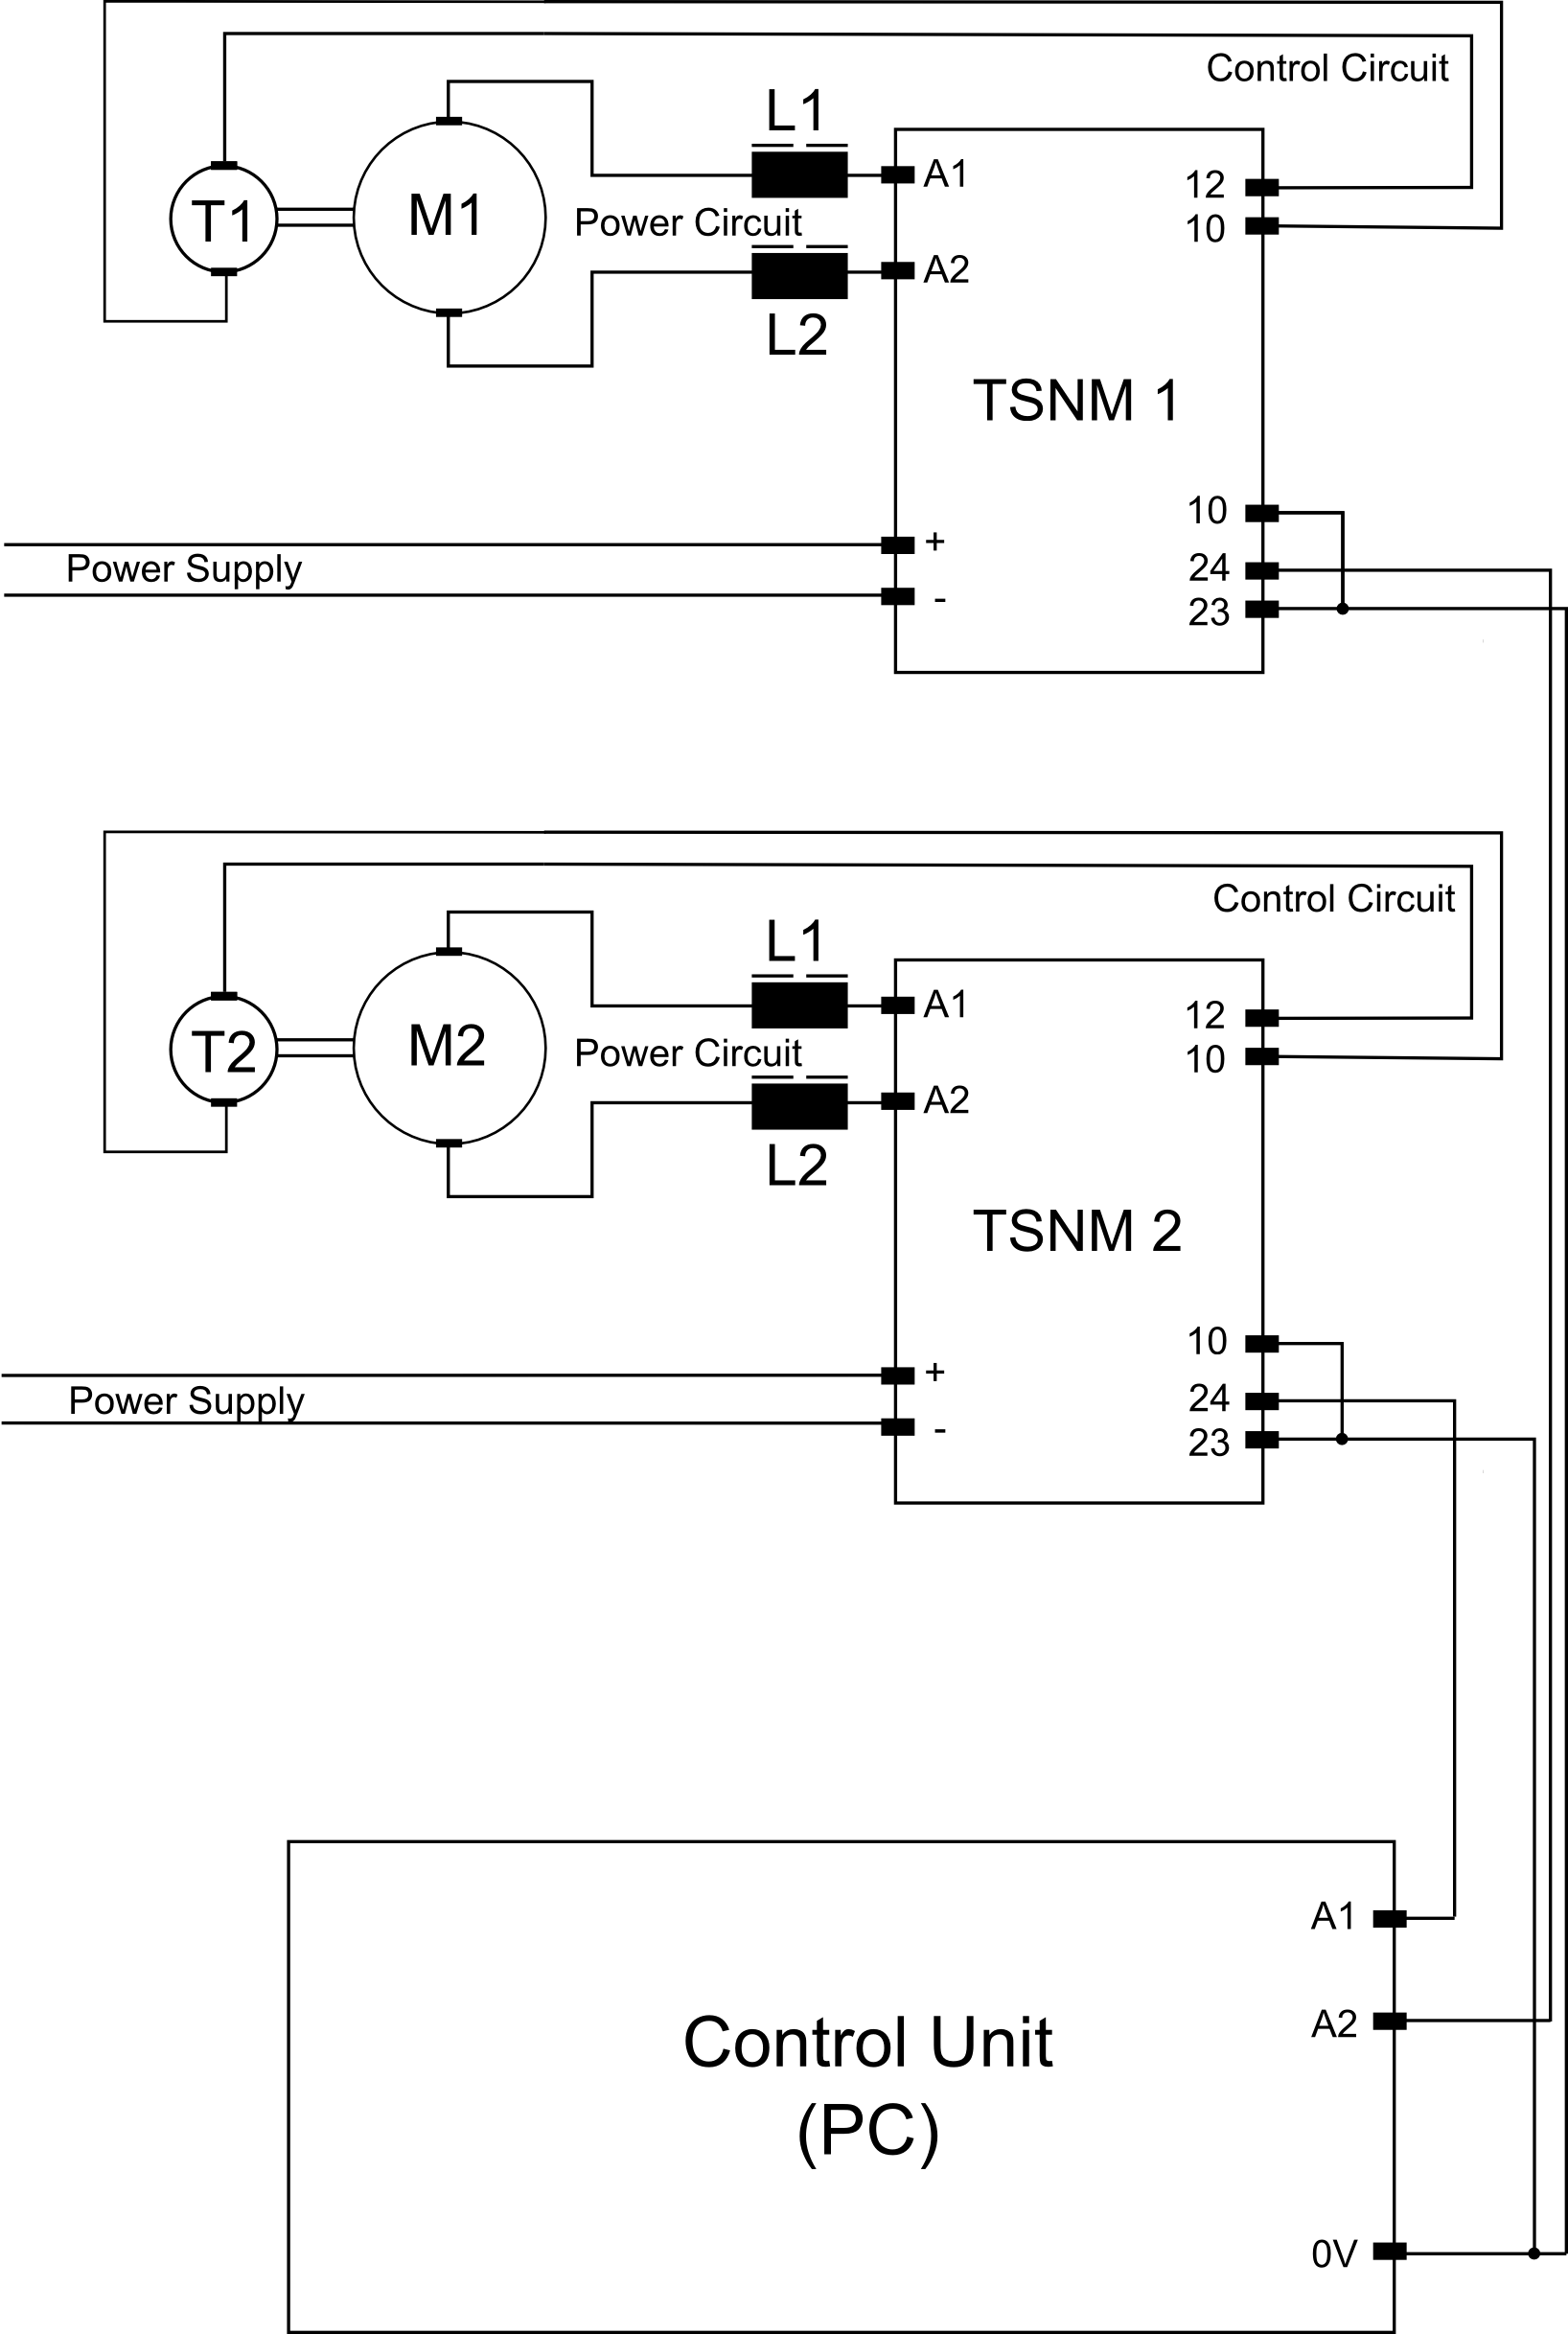
\includegraphics[width=\textwidth]{images/Schaltplan_Leistungselektronik.eps}
    \caption{Circuit Layout of Monochromator Control Electronics}
  \label{image:Schaltplan_Leistungselektronik}
\end{figure}



\clearpage
\bibliographystyle{dinateng}
\bibliography{bessy}
\end{document}
